\begin{table}[H]
\caption{Setups tested for inverting PROSAIL to derive GLAI and CCC using lookup-tables. All possible parameter combinations were tested and evaluated using retrieval performance on on-farm trials (Section \ref{subsec:on-farm-trials}).}
\label{tab:prosail-inv-settings}
\begin{tabular}{@{}lll@{}}
\toprule
\textbf{Parameter} & \textbf{Description}                                                                                     & \textbf{Tested Values}                                                                                                                                                \\ \midrule
cost function      & \begin{tabular}[c]{@{}l@{}}Cost function to compare\\observed and simulated\\spectra.\end{tabular}       & \begin{tabular}[c]{@{}l@{}}Mean Absolute Error,\\ Root Mean Squared Error,\\ Squared Sum of Differences\\ Contrast function\\suggested by~\cite{verrelst_optimizing_2014}\end{tabular} \\
lut-size           & Size of the LUT (number of spectra).                                                                     & 5000, 10000, 20000, 50000                                                                                                                                             \\
n-solutions        & \begin{tabular}[c]{@{}l@{}}Number of solutions in terms of\\smallest cost function values.\end{tabular} & 100, 1000, 5000                                                                                                                                                       \\
aggregation-method & \begin{tabular}[c]{@{}l@{}}Method to aggregate n-solutions\\into a single value.\end{tabular}           & Median, Mean, Weighted Mean                                                                                                                                           \\ \bottomrule
\end{tabular}
\end{table}

\begin{figure}[H]
    \centering
    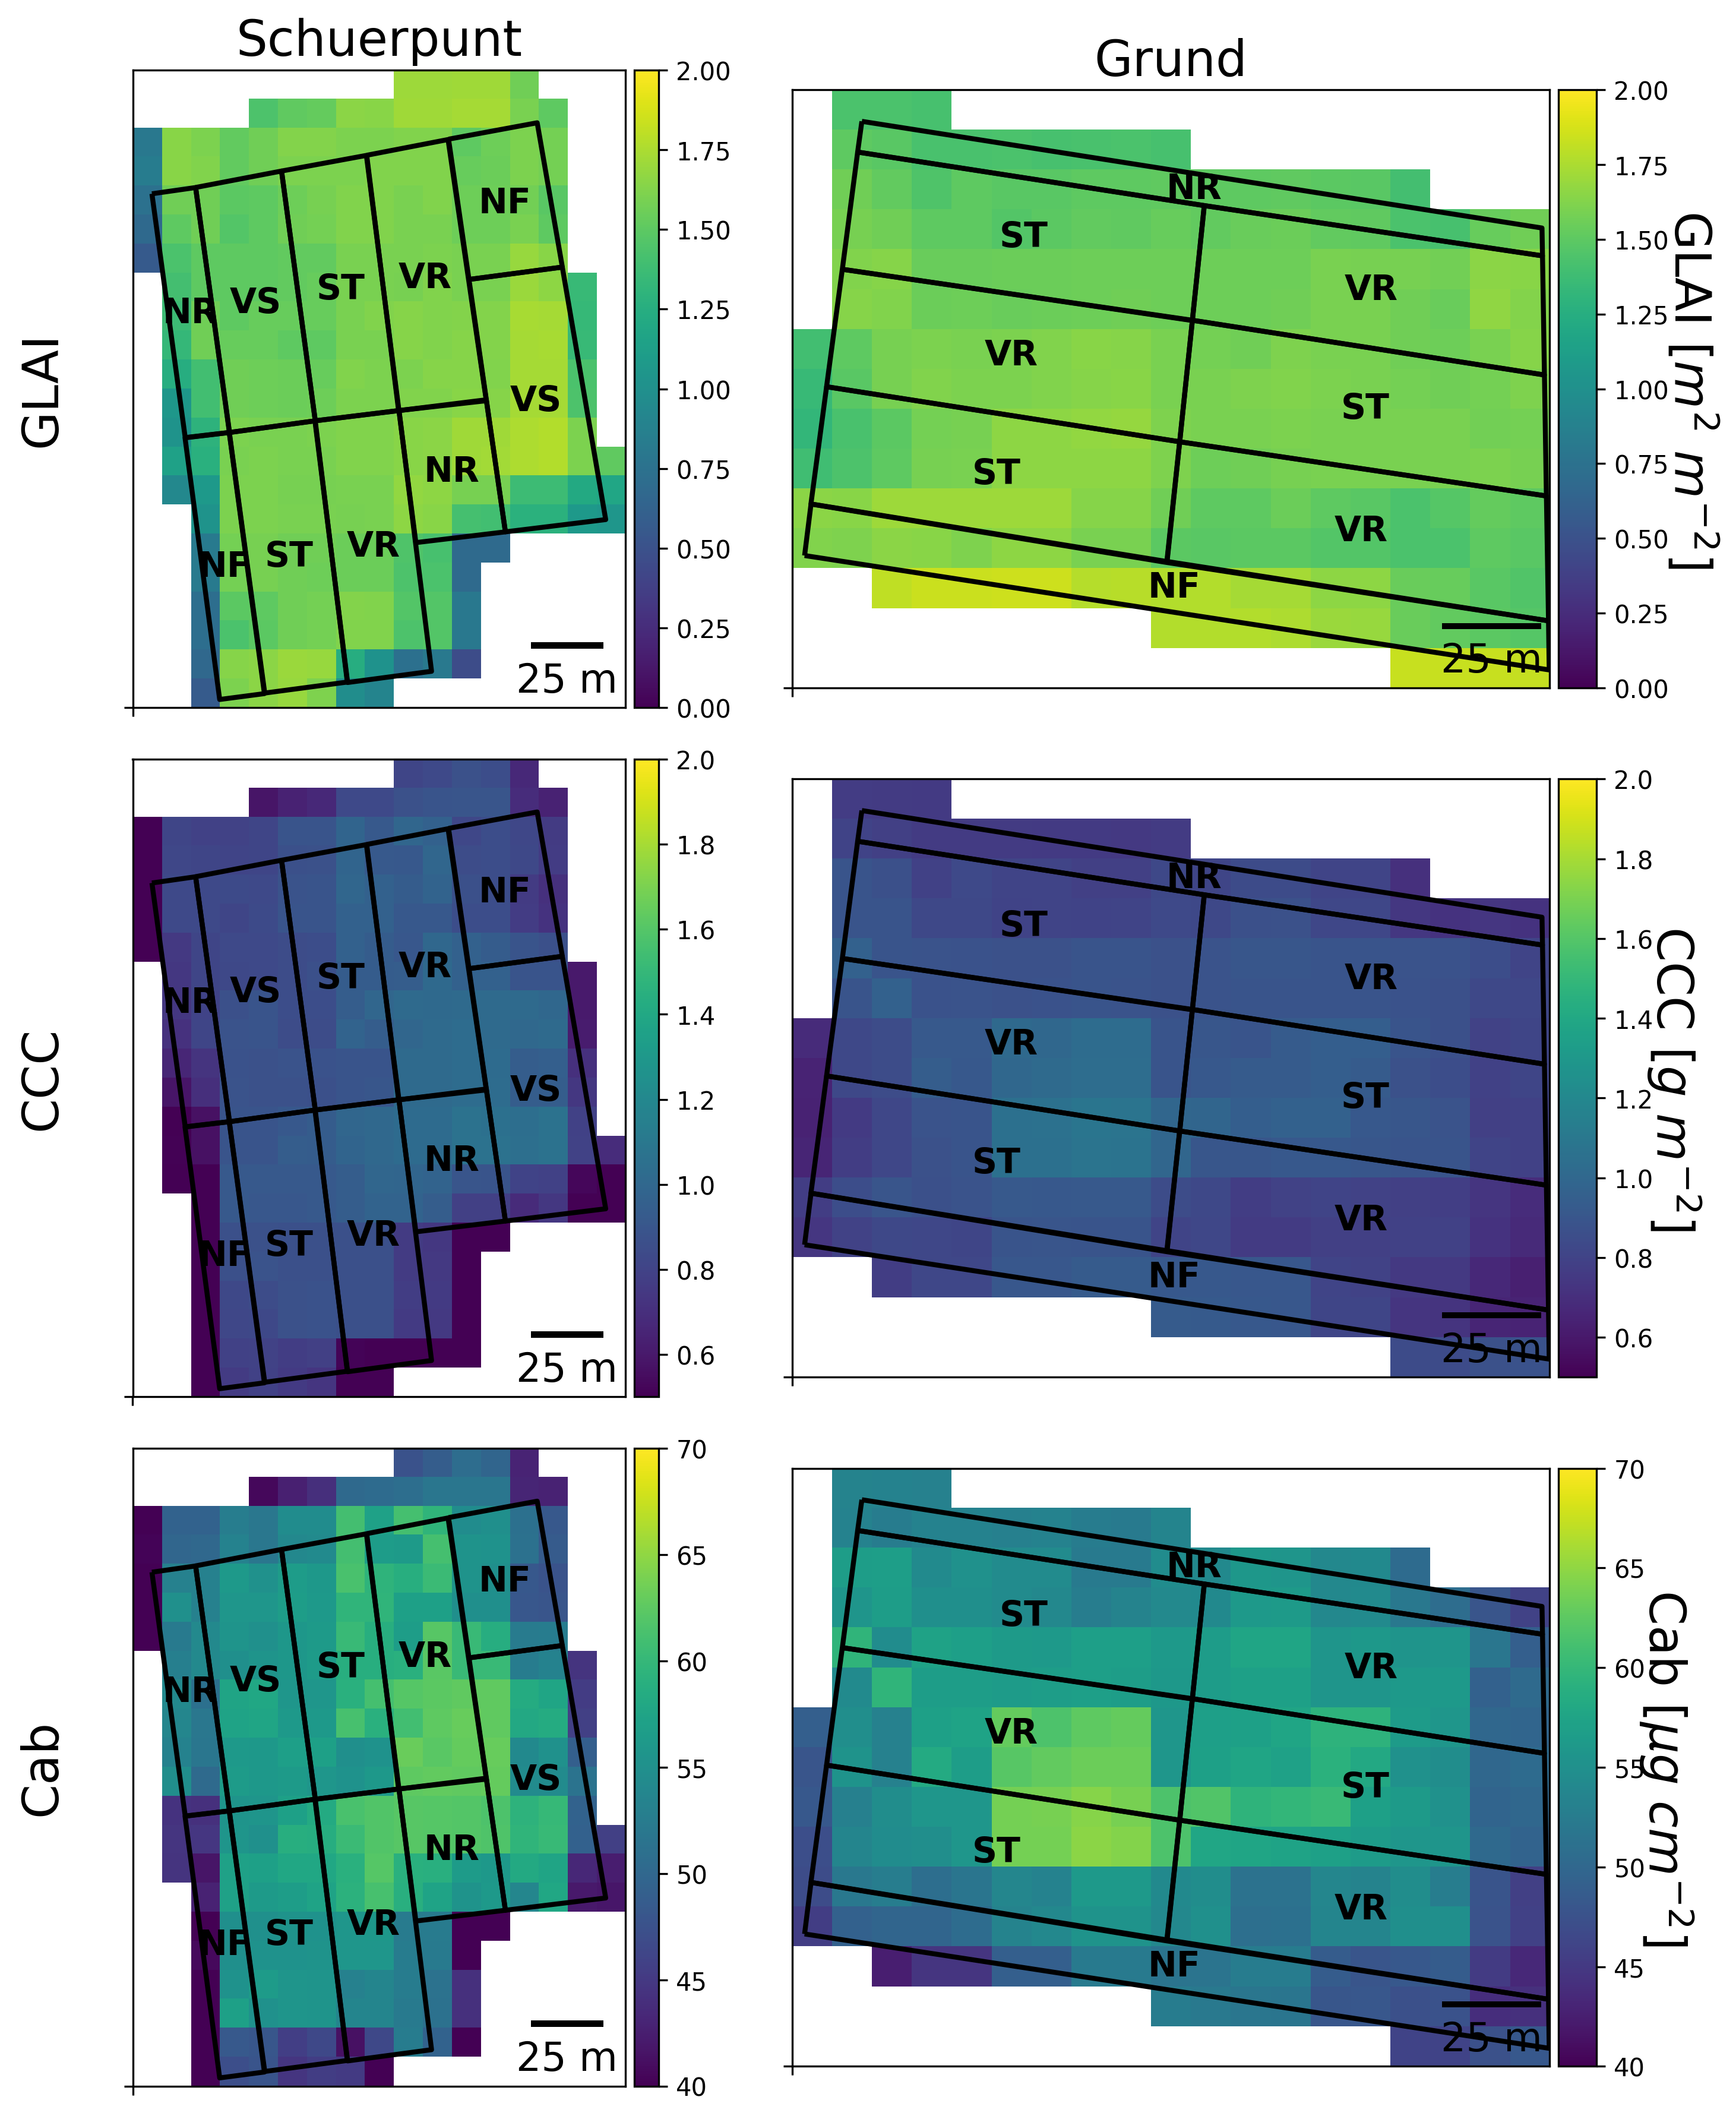
\includegraphics[width=0.9\textwidth]{SFF_2019_treatments_map.png}
    \caption[Maps of S2-derived GLAI (top), CCC (middle), and Cab (bottom) for the two winter wheat parcels studied at Swiss Future Farm acquired on April 20th, 2019. The treatment design by~\cite{argento_investigating_2022} is shown. The smaller treatment blocks at the field boundaries (width: 15 m) were excluded from our analysis. Explanation of the treatments: NR: nitrogen rich; NF: non-fertilized; ST: standard fertilization; VR: variable rate fertilization; VS: nitrogen fertilization suggested by Vista Remote Sensing in Geosciences GmbH.]{Maps of S2-derived GLAI (top), CCC (middle), and Cab (bottom) for the two winter wheat parcels studied at Swiss Future Farm acquired on April 20th, 2019. The treatment design by~\cite{argento_investigating_2022} is shown. The smaller treatment blocks at the field boundaries (width: 15 m) were excluded from our analysis. Explanation of the treatments: NR: nitrogen rich; NF: non-fertilized; ST: standard fertilization; VR: variable rate fertilization; VS: nitrogen fertilization suggested by Vista Remote Sensing in Geosciences GmbH.}
    \label{fig:appendix_sff_2019}
\end{figure}

% ----------------------------------- 2022 data -----------------------------

\begin{figure}[H]
    \centering
    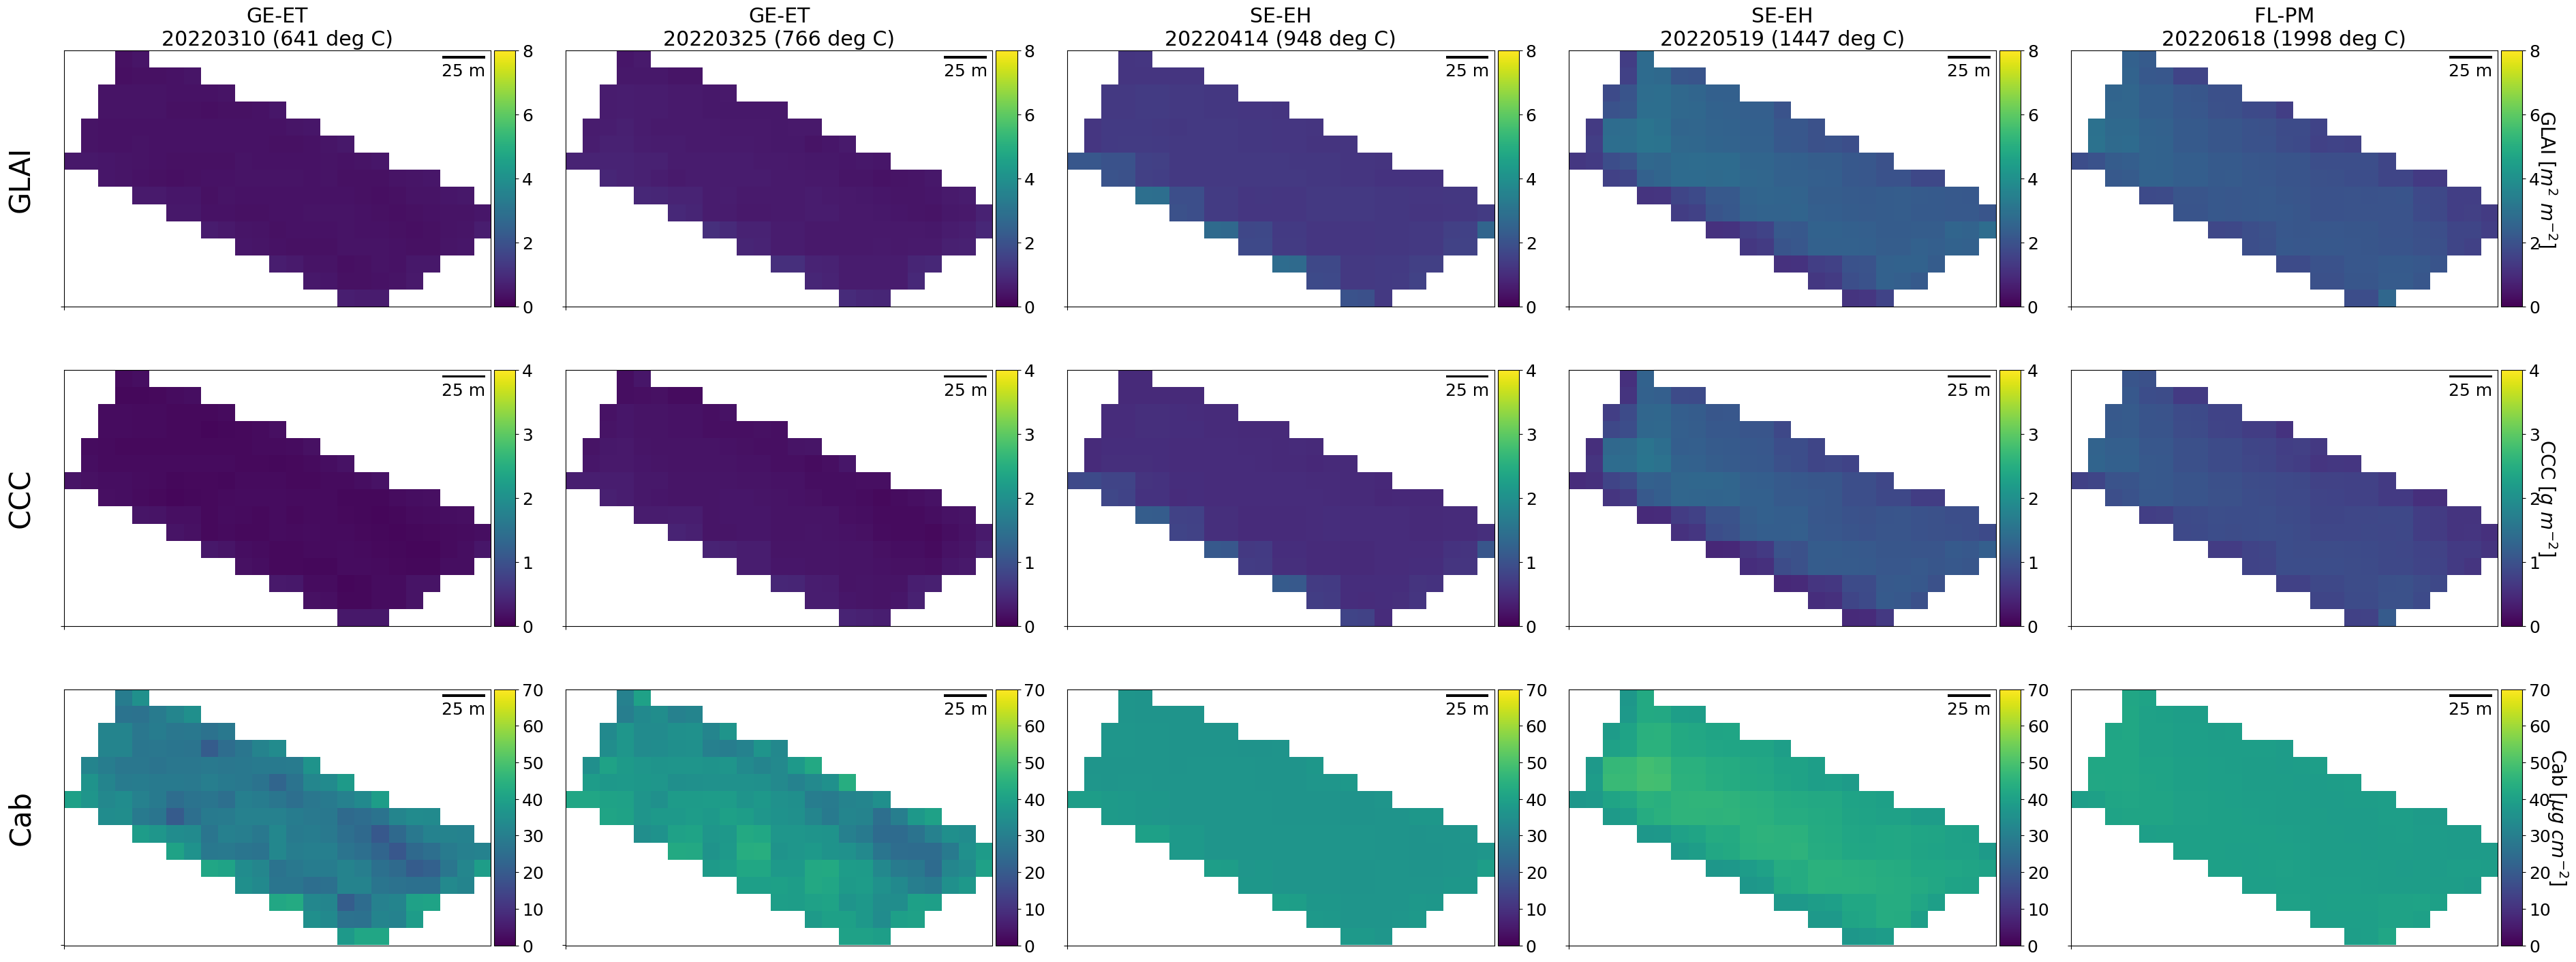
\includegraphics[width=1\textwidth]{Arenenberg_Broatefaeld_Trait_Maps.png}
    \caption[Maps of GLAI (top), CCC (middle), and Cab (bottom) derived from the best performing scenario (PHENO-AGDD) for Arenenberg (Broatefaeld). The maps are obtained from selected S2 overpasses depicting the three phenological macro stages of winter wheat (AGDD in brackets).]{Maps of GLAI (top), CCC (middle), and Cab (bottom) derived from the best performing scenario (PHENO-AGDD) for Arenenberg (Broatefaeld). The maps are obtained from selected S2 overpasses depicting the three phenological macro stages of winter wheat (AGDD in brackets).}
    \label{fig:appendix_arb_broatefaeld_2022}
\end{figure}

\begin{figure}[H]
    \centering
    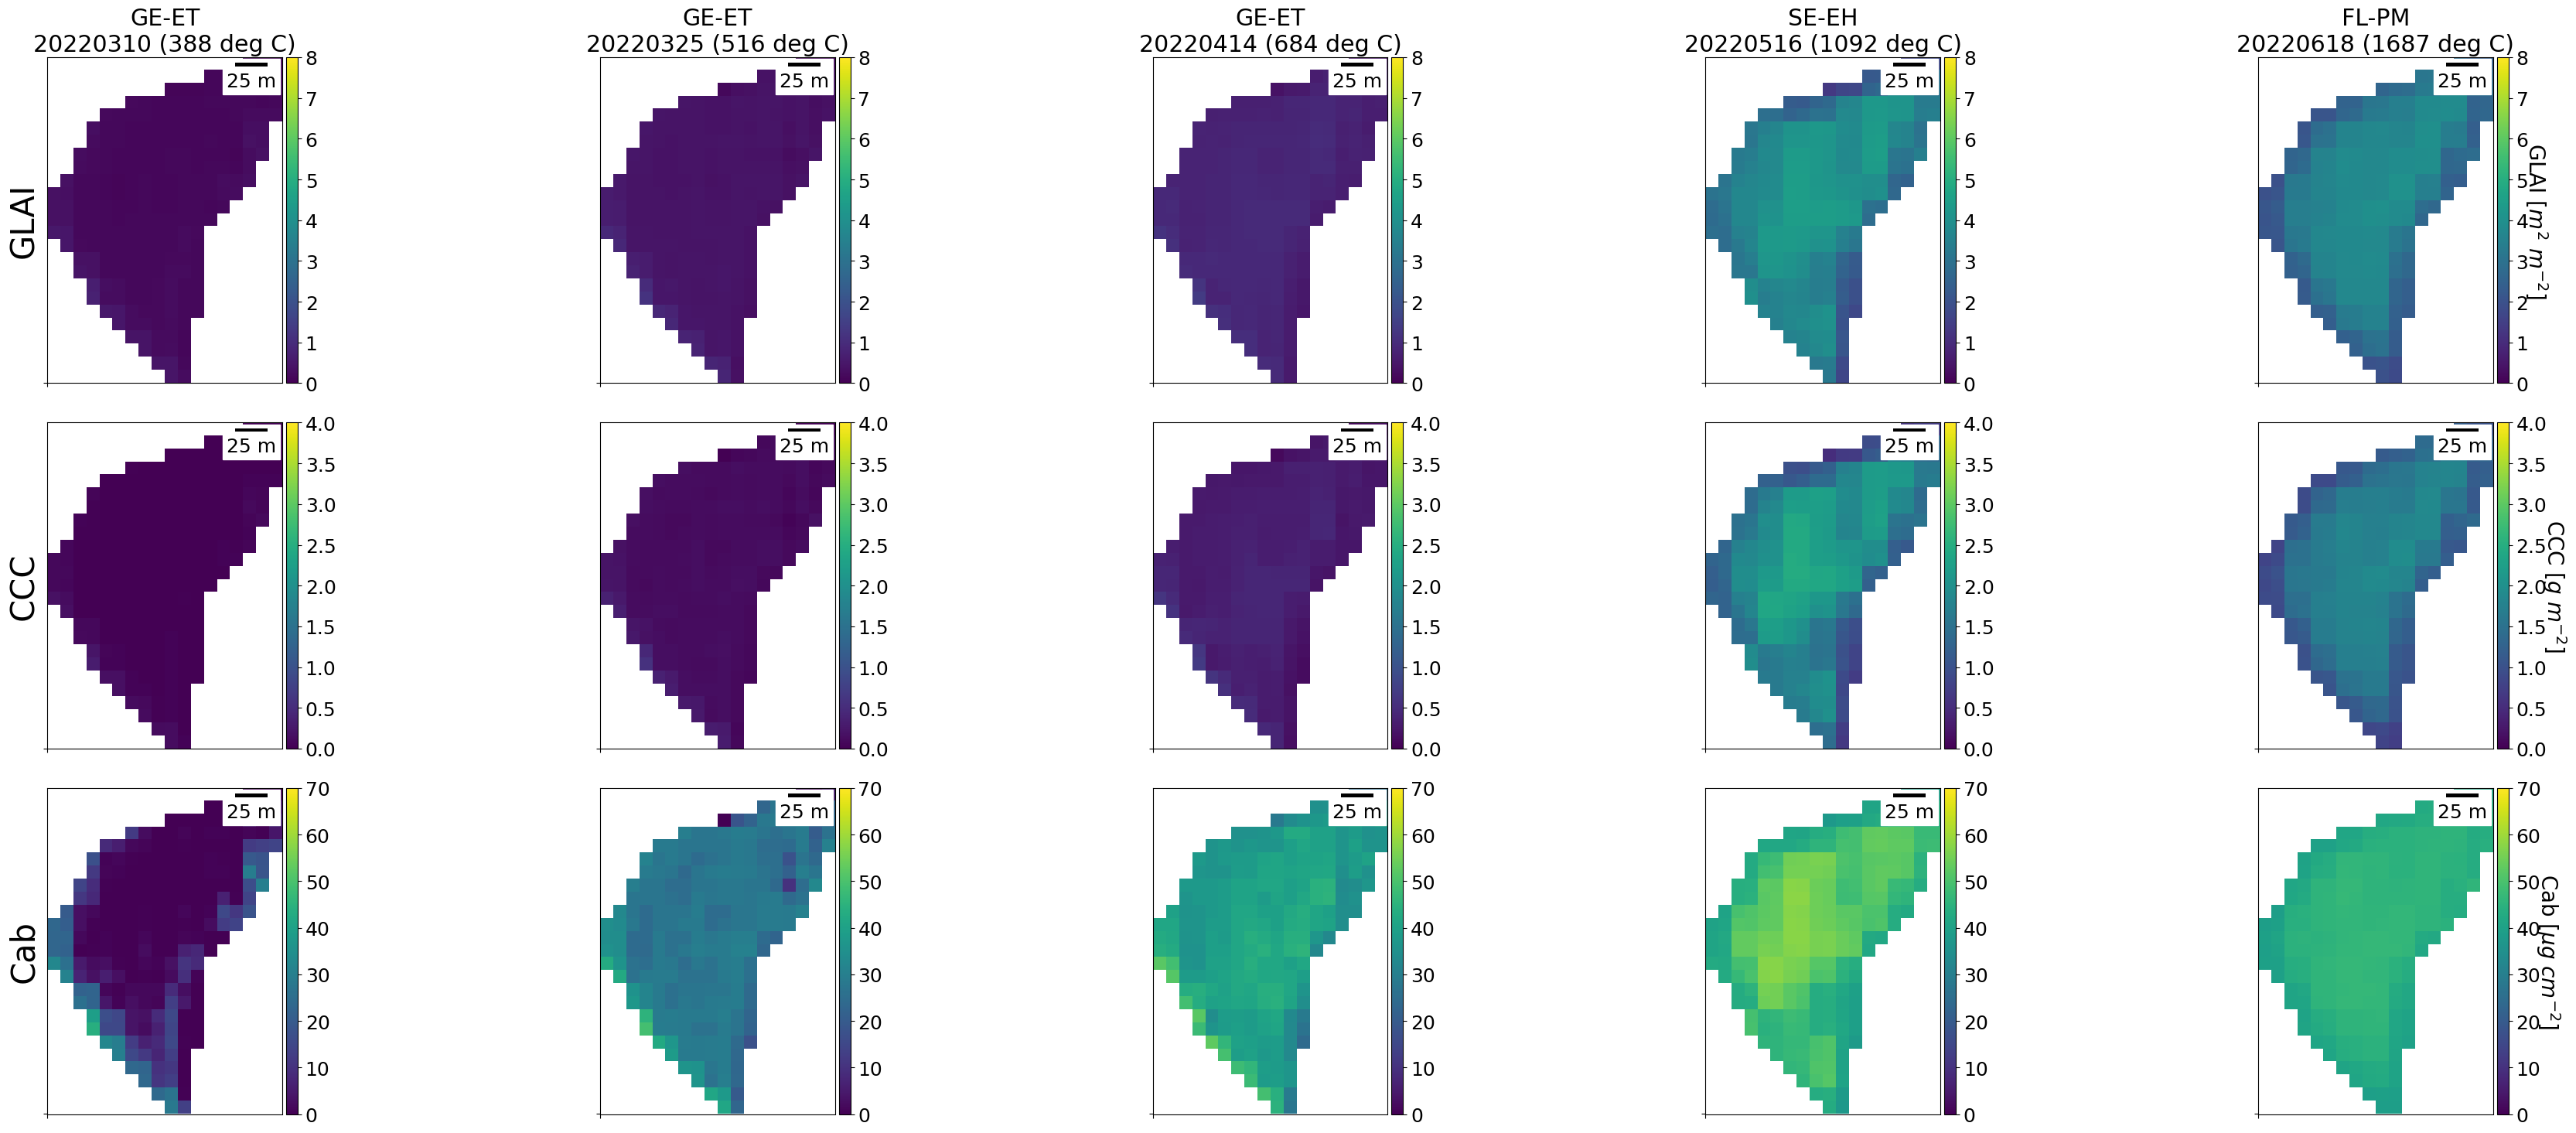
\includegraphics[width=1\textwidth]{Strickhof_Bramenwies_Trait_Maps.png}
    \caption[Maps of GLAI (top), CCC (middle), and Cab (bottom) derived from the best performing scenario (PHENO-AGDD) for Strickhof (Bramenwues). The maps are obtained from selected S2 overpasses depicting the three phenological macro stages of winter wheat (AGDD in brackets).]{Maps of GLAI (top), CCC (middle), and Cab (bottom) derived from the best performing scenario (PHENO-AGDD) for Strickhof (Bramenwues). The maps are obtained from selected S2 overpasses depicting the three phenological macro stages of winter wheat (AGDD in brackets).}
    \label{fig:appendix_sh_bramenwies_2022}
\end{figure}

\begin{figure}[H]
    \centering
    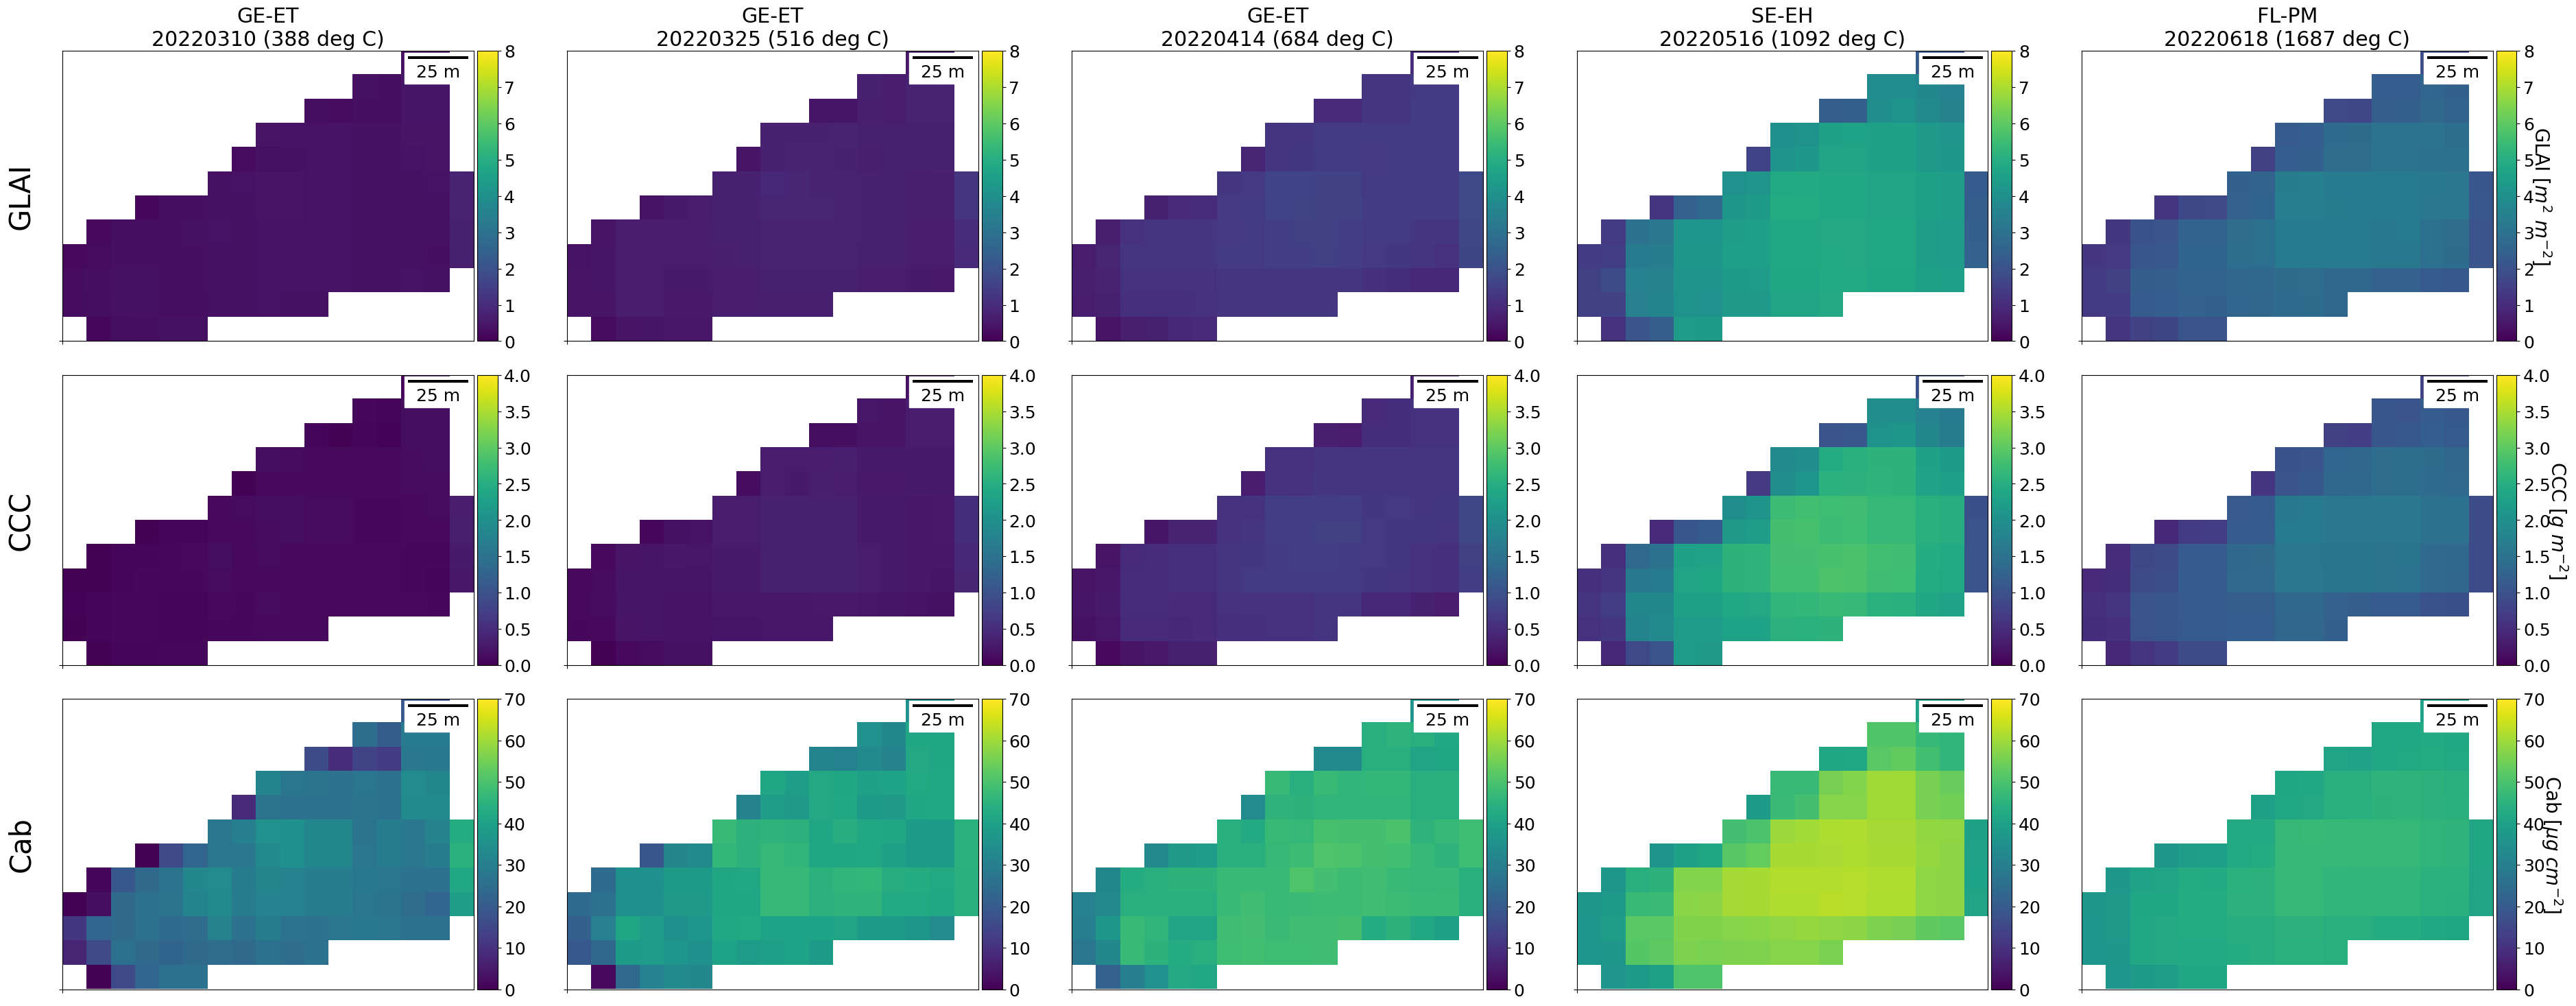
\includegraphics[width=1\textwidth]{Strickhof_Fluegenrain_Trait_Maps.png}
    \caption[Maps of GLAI (top), CCC (middle), and Cab (bottom) derived from the best performing scenario (PHENO-AGDD) for Strickhof (Fluegenrain). The maps are obtained from selected S2 overpasses depicting the three phenological macro stages of winter wheat (AGDD in brackets).]{Maps of GLAI (top), CCC (middle), and Cab (bottom) derived from the best performing scenario (PHENO-AGDD) for Strickhof (Fluegenrain). The maps are obtained from selected S2 overpasses depicting the three phenological macro stages of winter wheat (AGDD in brackets).}
    \label{fig:appendix_sh_fluegenrain_2022}
\end{figure}

\begin{figure}[H]
    \centering
    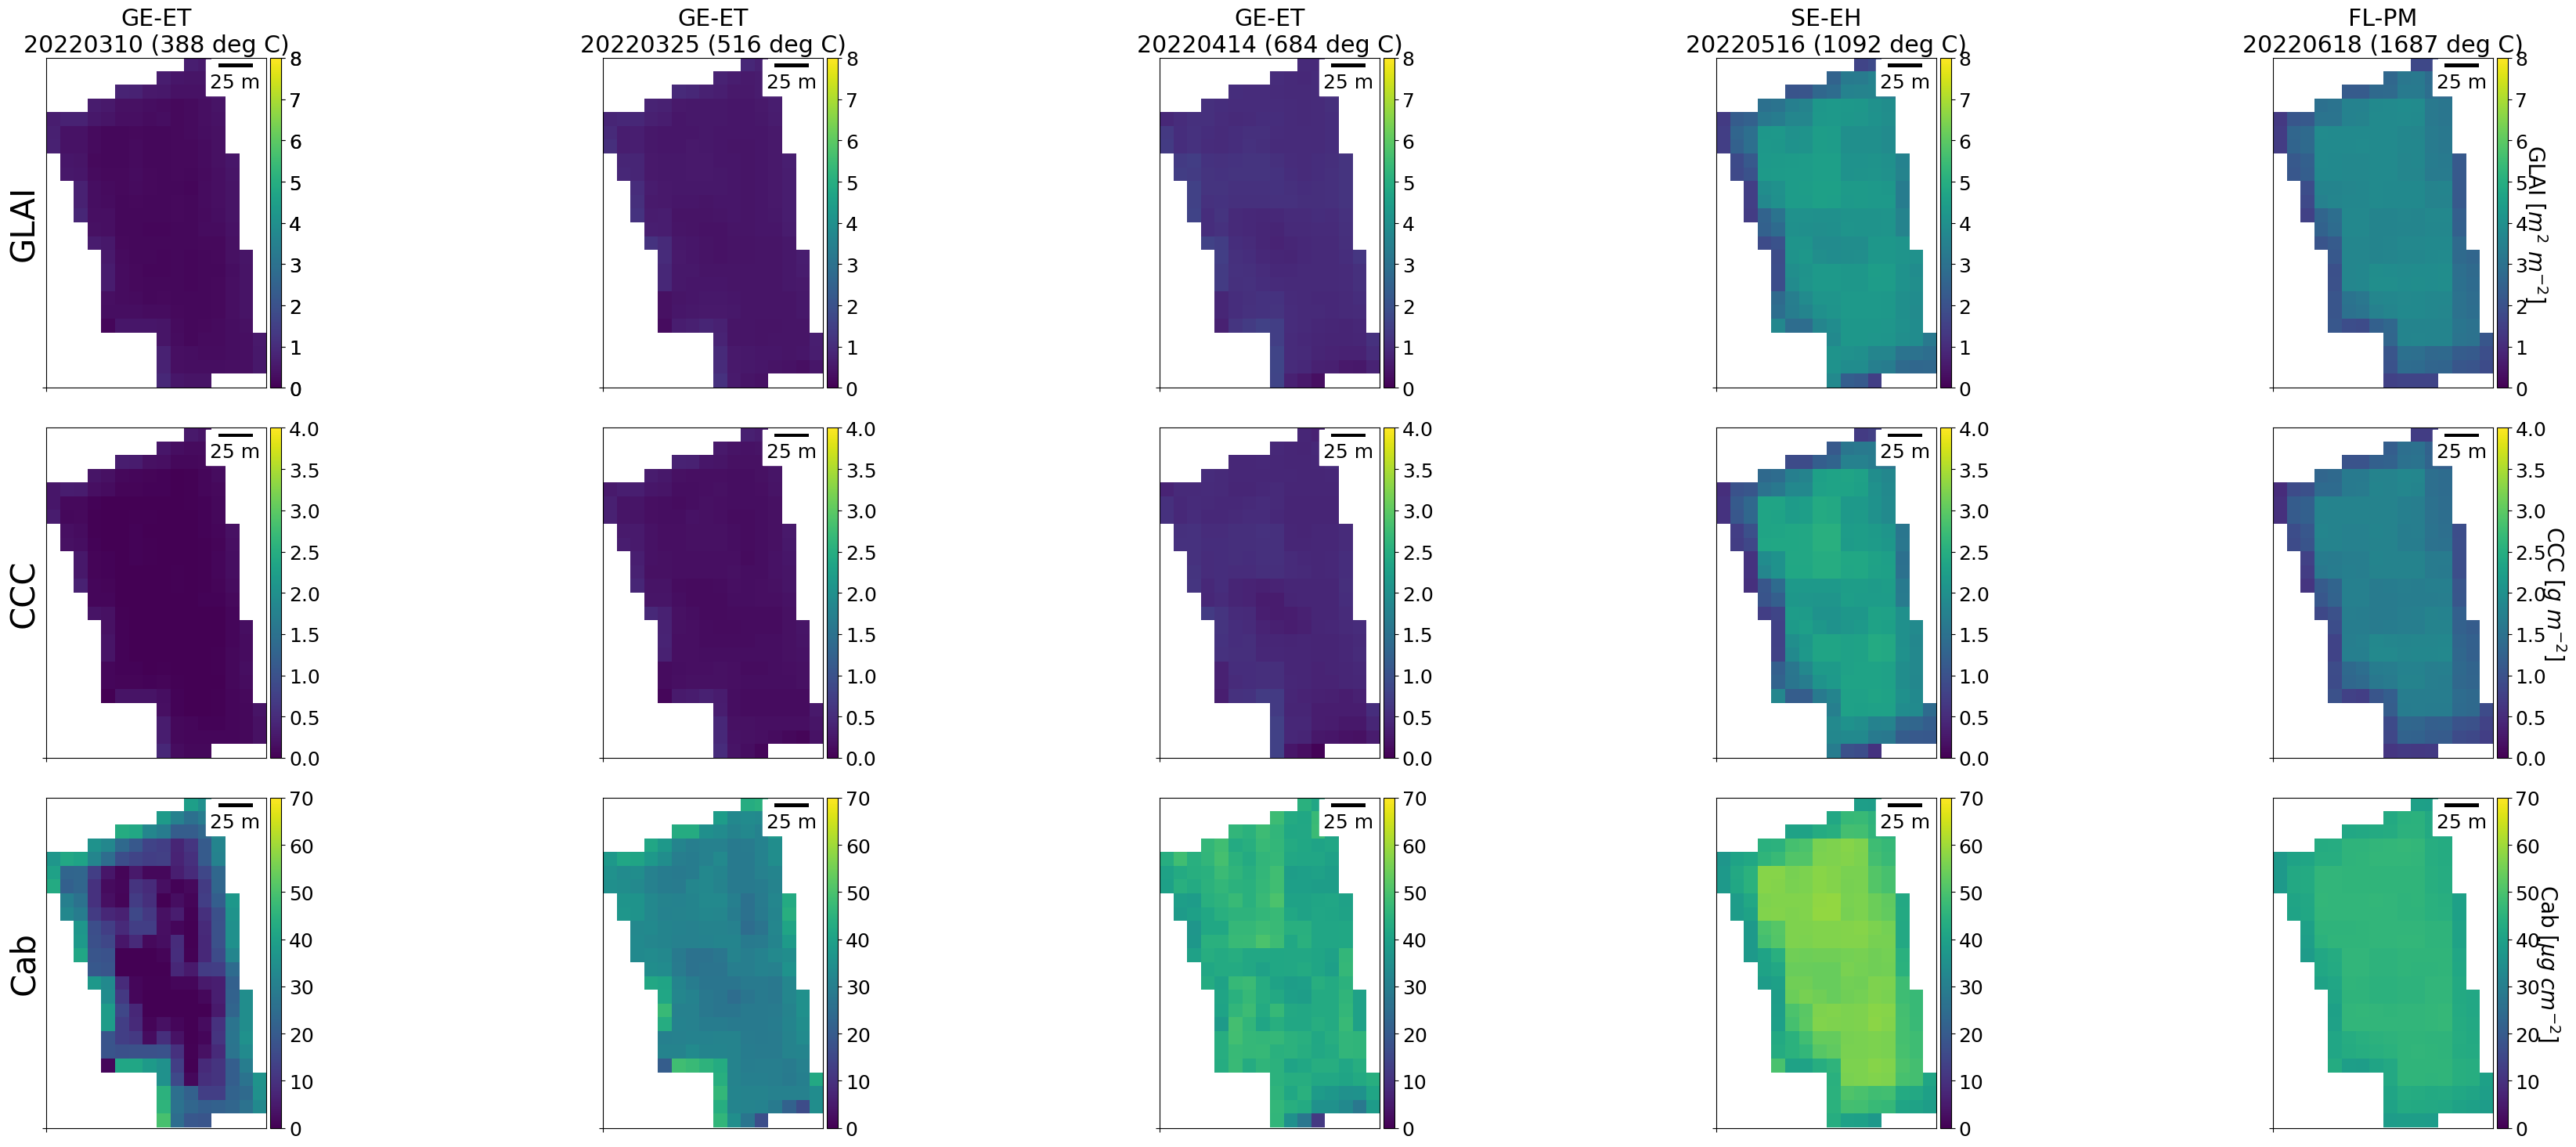
\includegraphics[width=1\textwidth]{Strickhof_Hohrueti_Trait_Maps.png}
    \caption[Maps of GLAI (top), CCC (middle), and Cab (bottom) derived from the best performing scenario (PHENO-AGDD) for Strickhof (Hohrueti). The maps are obtained from selected S2 overpasses depicting the three phenological macro stages of winter wheat (AGDD in brackets).]{Maps of GLAI (top), CCC (middle), and Cab (bottom) derived from the best performing scenario (PHENO-AGDD) for Strickhof (Hohrueti). The maps are obtained from selected S2 overpasses depicting the three phenological macro stages of winter wheat (AGDD in brackets).}
    \label{fig:appendix_sh_hohrueti_2022}
\end{figure}

\begin{figure}[H]
    \centering
    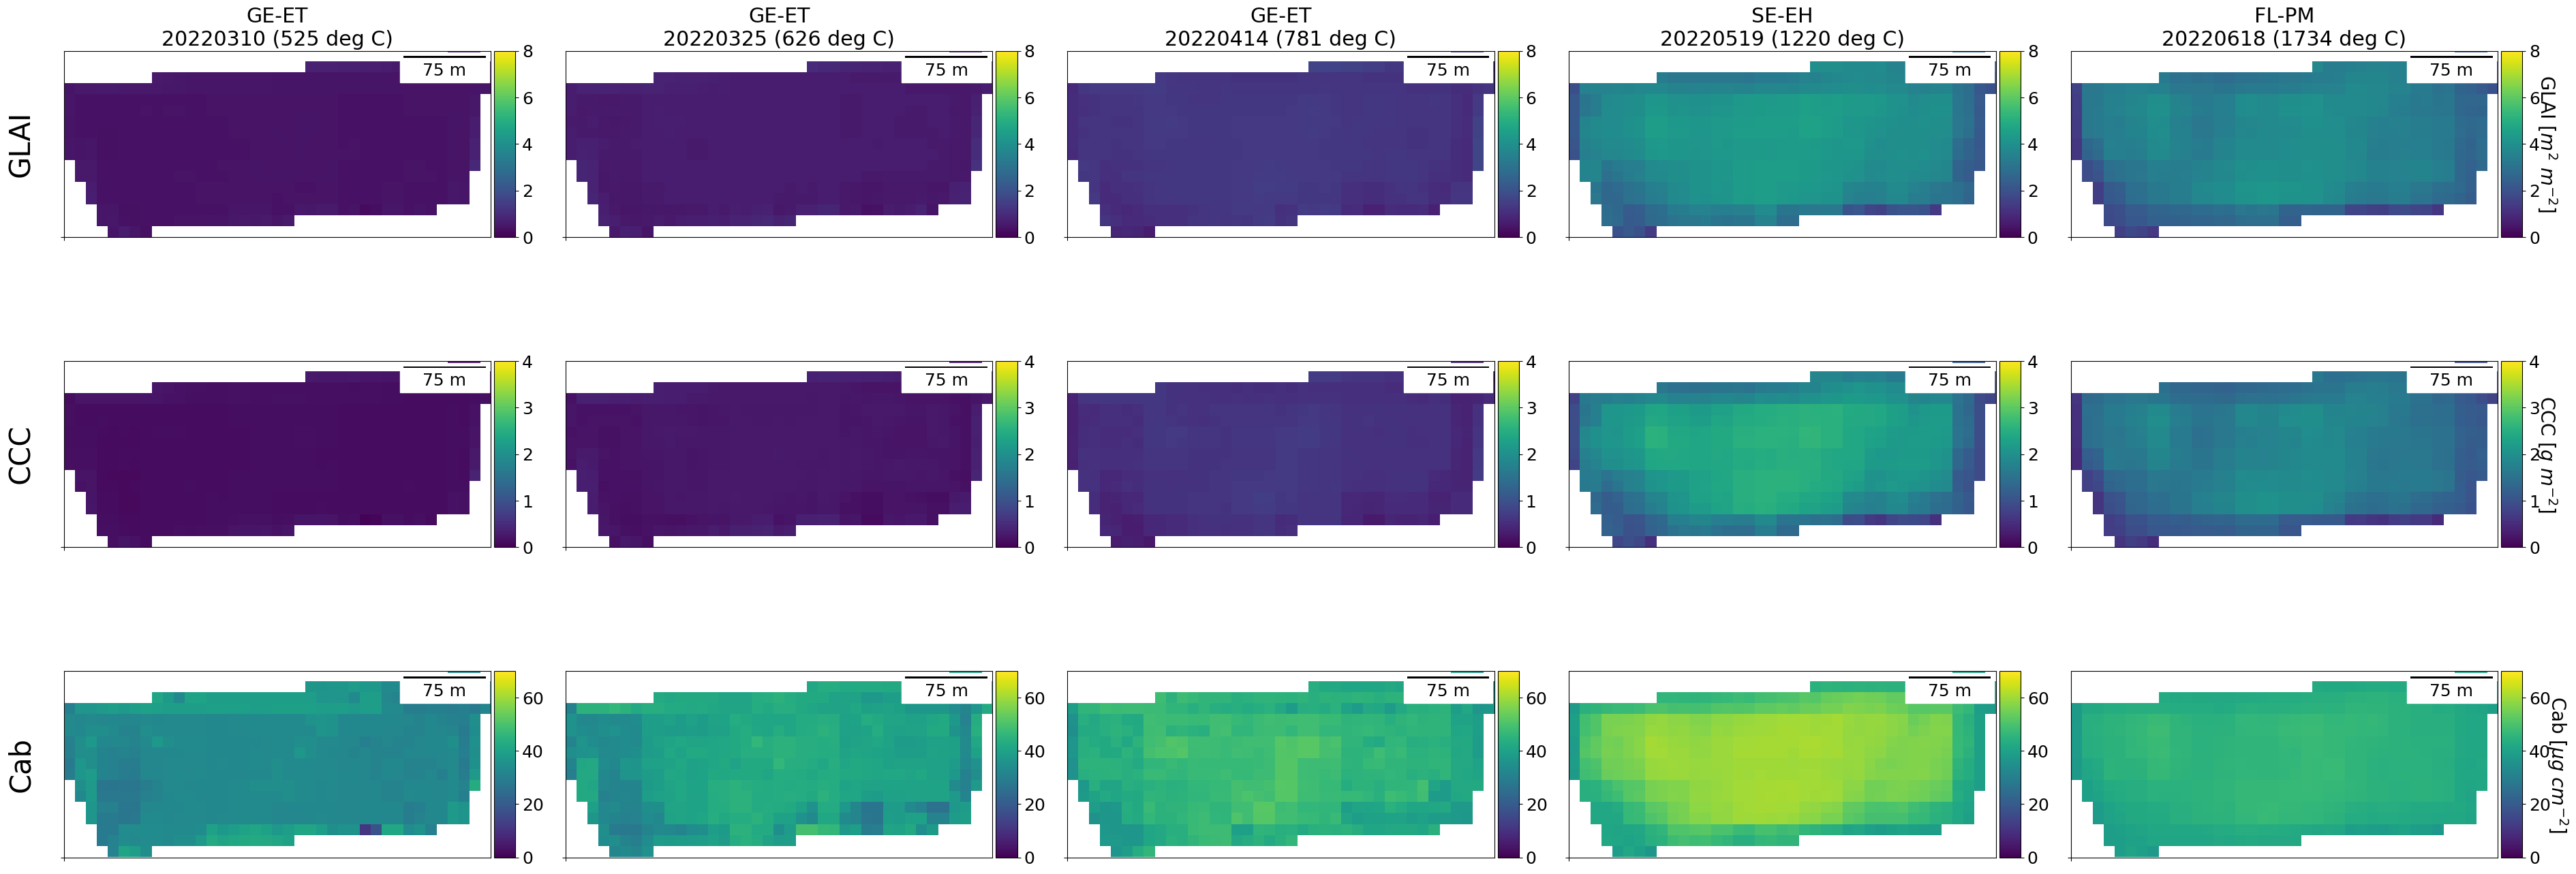
\includegraphics[width=1\textwidth]{SwissFutureFarm_Altkloster_Trait_Maps.png}
    \caption[Maps of GLAI (top), CCC (middle), and Cab (bottom) derived from the best performing scenario (PHENO-AGDD) for Swiss Future Farm (Altkloster). The maps are obtained from selected S2 overpasses depicting the three phenological macro stages of winter wheat (AGDD in brackets).]{Maps of GLAI (top), CCC (middle), and Cab (bottom) derived from the best performing scenario (PHENO-AGDD) for Swiss Future Farm (Altkloster). The maps are obtained from selected S2 overpasses depicting the three phenological macro stages of winter wheat (AGDD in brackets).}
    \label{fig:appendix_sff_altkloster_2022}
\end{figure}

\begin{figure}[H]
    \centering
    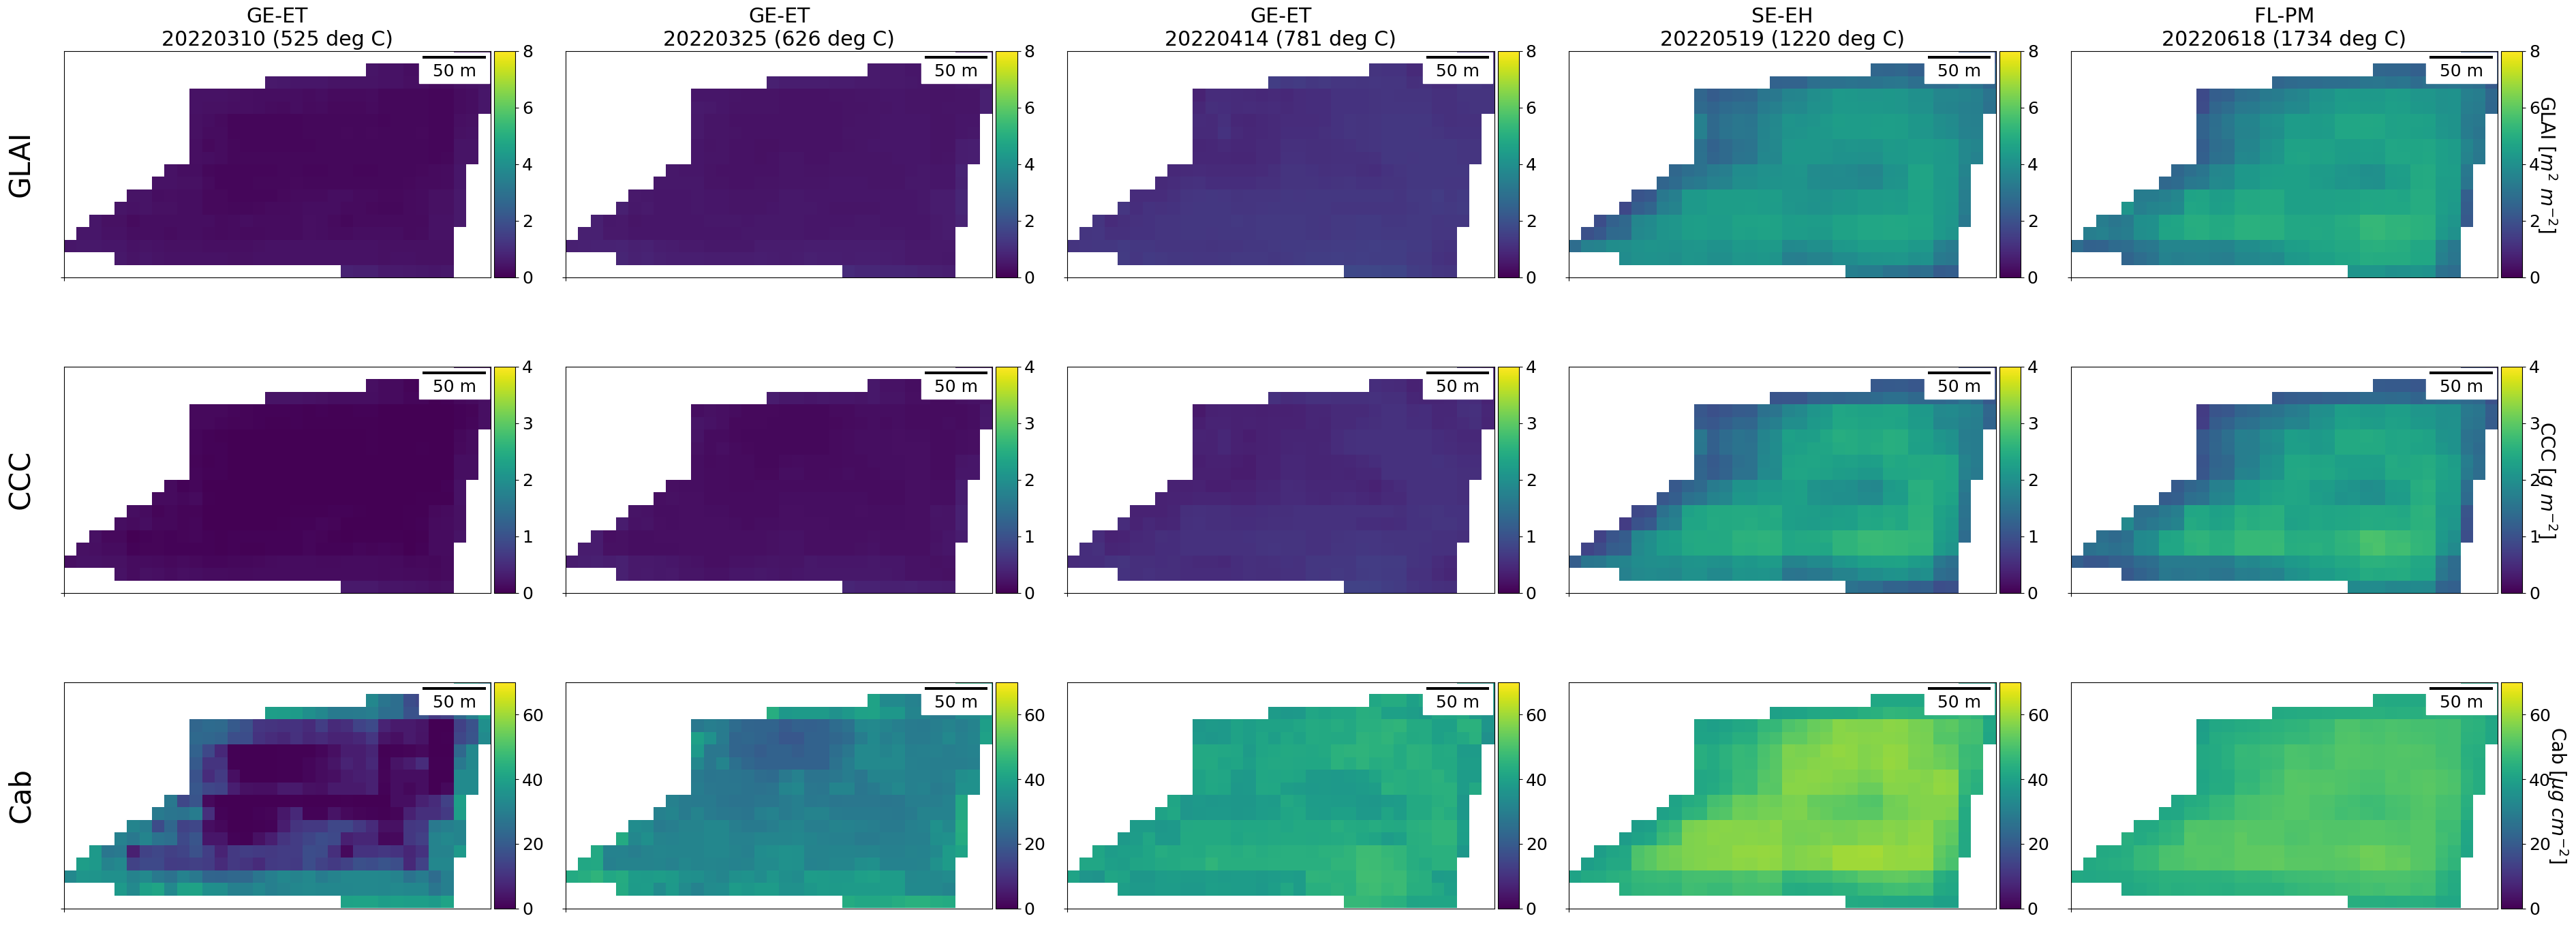
\includegraphics[width=1\textwidth]{SwissFutureFarm_Ruetteli_Trait_Maps.png}
    \caption[Maps of GLAI (top), CCC (middle), and Cab (bottom) derived from the best performing scenario (PHENO-AGDD) for Swiss Future Farm (Ruetteli). The maps are obtained from selected S2 overpasses depicting the three phenological macro stages of winter wheat (AGDD in brackets).]{Maps of GLAI (top), CCC (middle), and Cab (bottom) derived from the best performing scenario (PHENO-AGDD) for Swiss Future Farm (Ruetteli). The maps are obtained from selected S2 overpasses depicting the three phenological macro stages of winter wheat (AGDD in brackets).}
    \label{fig:appendix_sff_ruetteli_2022}
\end{figure}